\documentclass[12pt,letterpaper]{article}
\usepackage[utf8]{inputenc}
\usepackage[spanish]{babel}
\usepackage{graphicx}
\usepackage[left=2cm,right=2cm,top=2cm,bottom=2cm]{geometry}
\usepackage{graphicx} % figuras
% \usepackage{subfigure} % subfiguras
\usepackage{float} % para usar [H]
\usepackage{amsmath}
%\usepackage{txfonts}
\usepackage{stackrel} 
\usepackage{multirow}
\usepackage{enumerate} % enumerados
\renewcommand{\labelitemi}{$-$}
\renewcommand{\labelitemii}{$\cdot$}
% \author{}
% \title{Caratula}
\begin{document}

% Fancy Header and Footer
% \usepackage{fancyhdr}
% \pagestyle{fancy}
% \cfoot{}
% \rfoot{\thepage}
%

% \usepackage[hidelinks]{hyperref} % CREA HYPERVINCULOS EN INDICE

% \author{}
\title{Caratula}

\begin{titlepage}
\begin{center}
\large{UNIVERSIDAD PRIVADA-DE-TACNA}\\
\vspace*{-0.025in}
\begin{figure}[htb]
\begin{center}

\includegraphics[width=8cm]{./Imagenes/logo}
\end{center}
\end{figure}
\vspace*{0.15in}
INGENIERIA DE SISTEMAS  \\

\vspace*{0.5in}
\begin{large}
TITULO:\\
\end{large}

\vspace*{0.1in}
\begin{Large}
\textbf{Elaboración de Dashboards en Power BI} \\
\end{Large}

\vspace*{0.3in}
\begin{Large}
\textbf{CURSO:} \\
\end{Large}

\vspace*{0.1in}
\begin{large}
Inteligencia de Negocios\\
\end{large}

\vspace*{0.3in}
\begin{Large}
\textbf{DOCENTE(ING):} \\
\end{Large}

\vspace*{0.1in}
\begin{large}
 Patrick Cuadros Quiroga\\
\end{large}

\vspace*{0.2in}
\vspace*{0.1in}
\begin{large}
Integrante: \\
\begin{flushleft}
Rivas Rios, Marko Antonio          	\hfill	(2016054461) \\

\end{flushleft}
\end{large}
\end{center}

\end{titlepage}


\tableofcontents % INDICE
\thispagestyle{empty} % INDICE SIN NUMERO
\newpage
\setcounter{page}{1} % REINICIAR CONTADOR DE PAGINAS DESPUES DEL INDICE

\section{Proceso} 

\begin{itemize}
	\item Cuadro de dialogo Navegador
	\begin{center}
	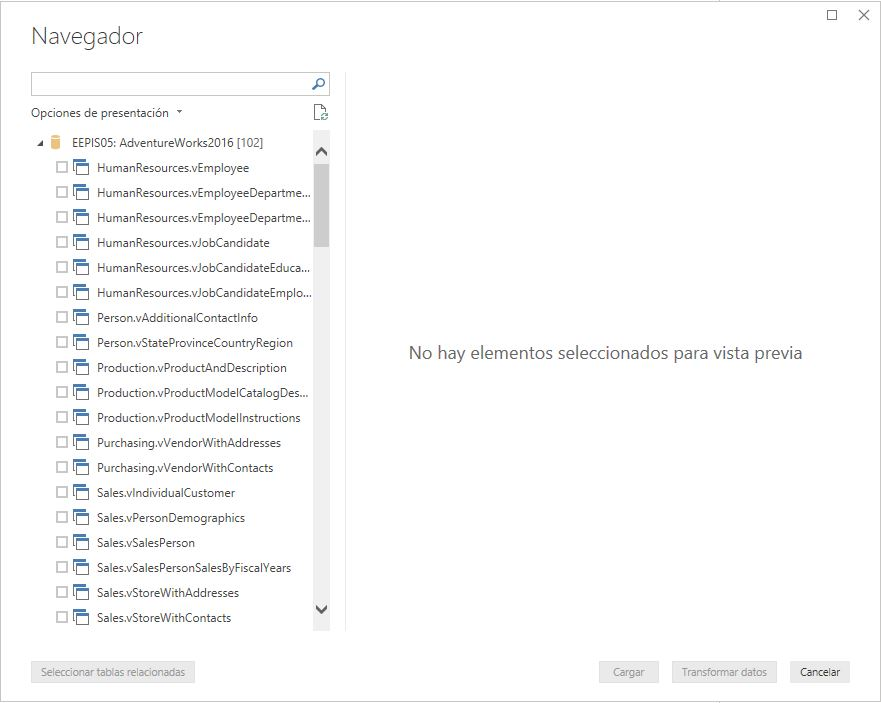
\includegraphics[width=10cm]{./Imagenes/Captura1} 
	\end{center}
\end{itemize} 

\begin{itemize}
	\item Seleccionando la vista Sales.vSalesPerson
	\begin{center}
	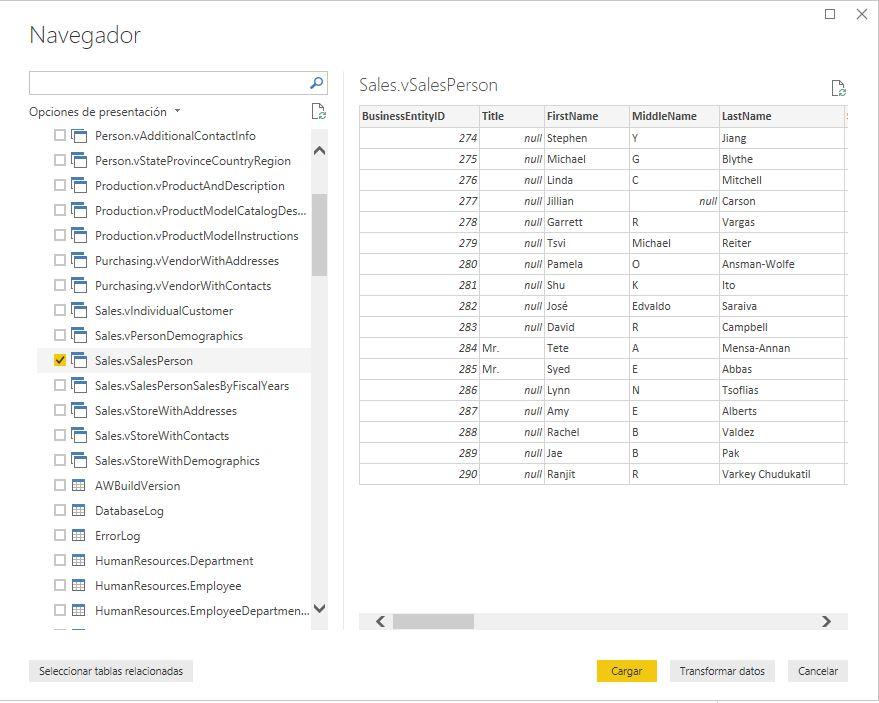
\includegraphics[width=10cm]{./Imagenes/Captura2} 
	\end{center}
\end{itemize} 

\begin{itemize}
	\item Seleccionando la vista Sales.vStoreWithDemographics
	\begin{center}
	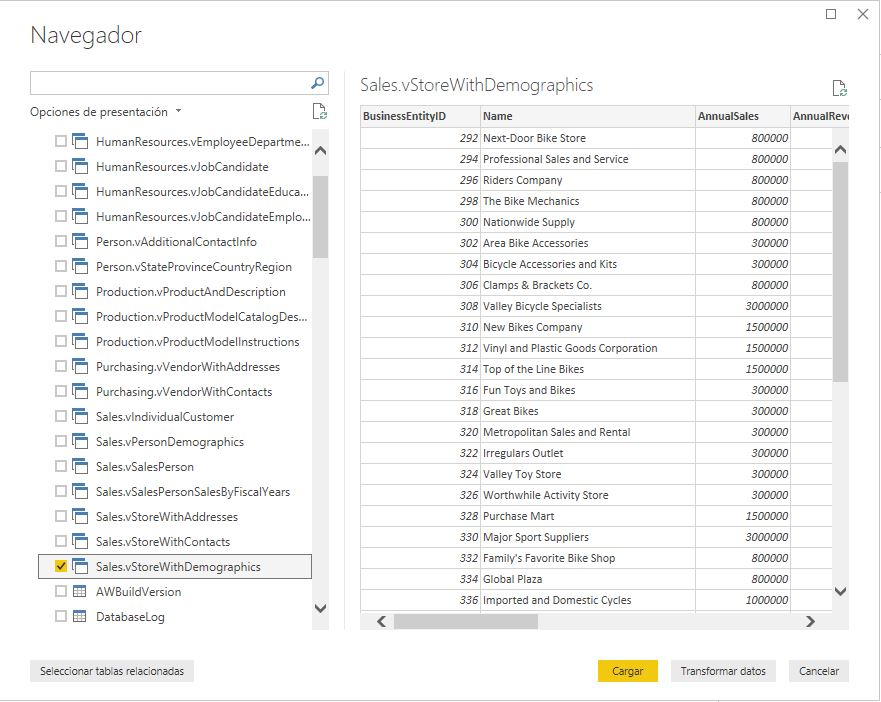
\includegraphics[width=10cm]{./Imagenes/Captura3} 
	\end{center}
\end{itemize} 

\begin{itemize}
	\item Opciones Avanzadas de obtener datos SQL Server, en la casilla sentencia SQL
	\begin{center}
	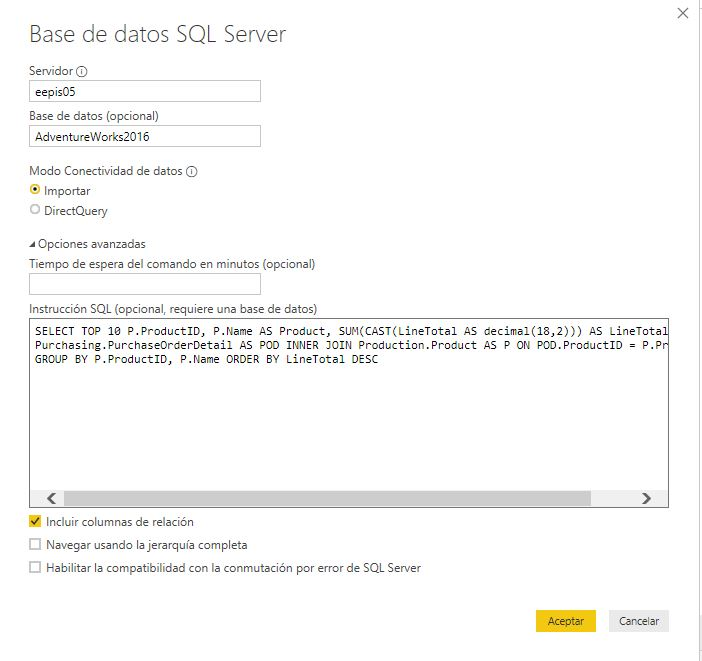
\includegraphics[width=10cm]{./Imagenes/Captura4} 
	\end{center}
\end{itemize} 

\begin{itemize}
	\item Panel Campos con las vistas seleccionadas
	\begin{center}
	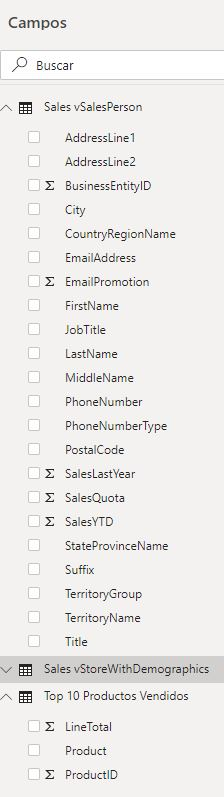
\includegraphics[width=5cm]{./Imagenes/Captura4-5} 
	\end{center}
\end{itemize} 

\begin{itemize}
	\item Reporte con Graficos Power Bi
	\begin{center}
	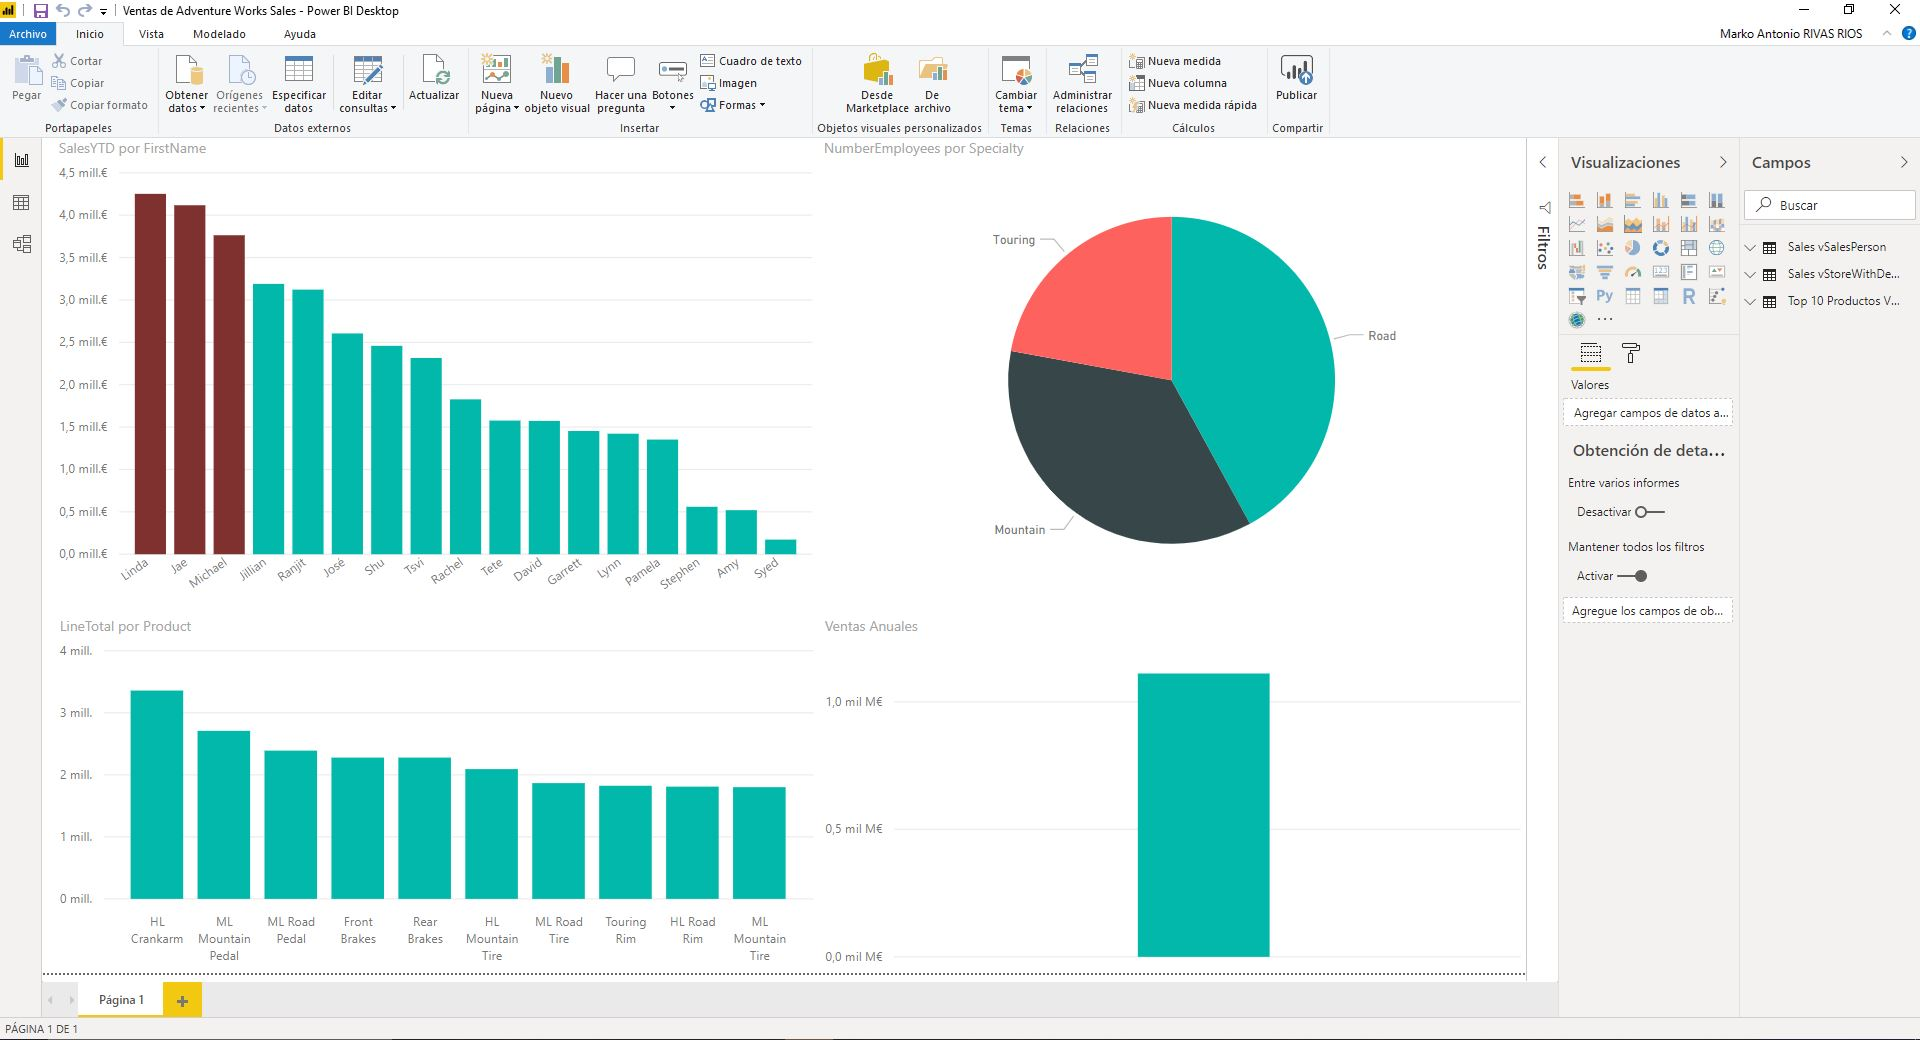
\includegraphics[width=13cm]{./Imagenes/Captura5} 
	\end{center}
\end{itemize} 

\begin{itemize}
	\item Reporte con Graficos portal de Power Bi 
	\begin{center}
	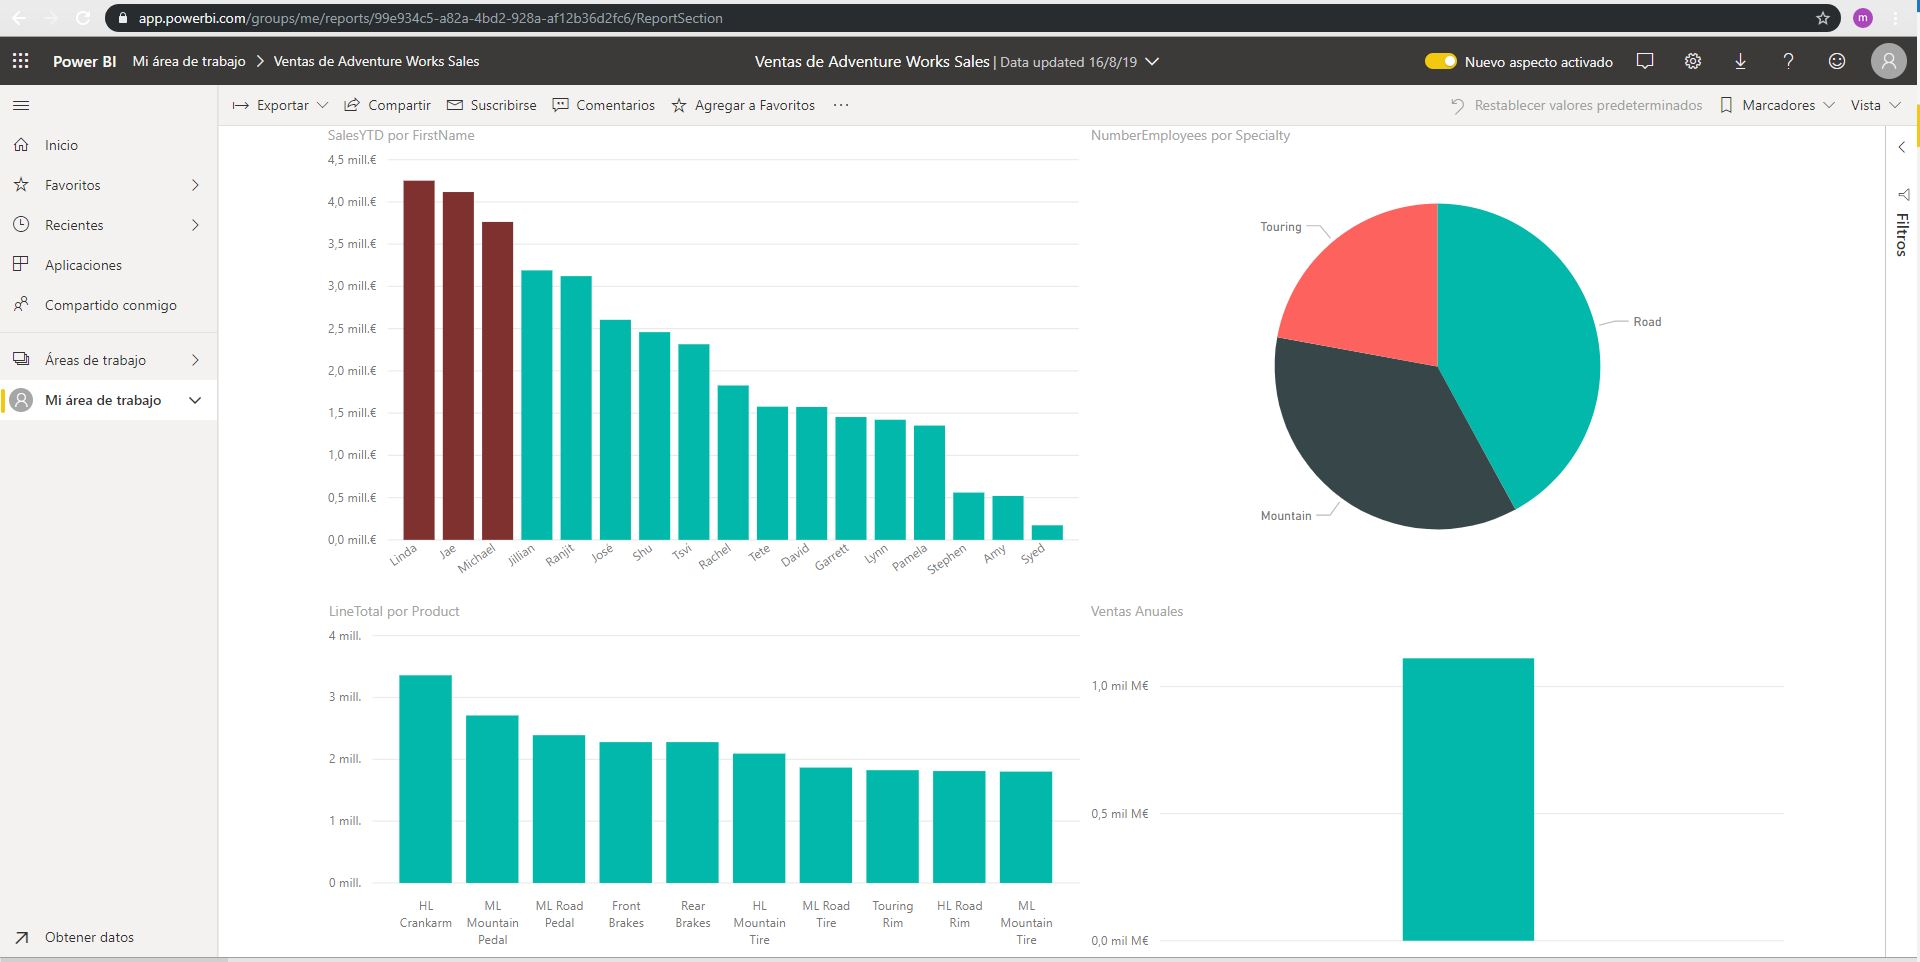
\includegraphics[width=13cm]{./Imagenes/Captura6} 
	\end{center}
\end{itemize} 
\begin{itemize}
	\item  Ruta del informe en el Portal de Power BI :
	\textbf{} \\
	https://app.powerbi.com/groups/me/reports/99e934c5-a82a-4bd2-928a-af12b36d2fc6/ReportSection
\end{itemize} 





\end{document}
